\documentclass[conference]{styles/acmsiggraph}

\usepackage{comment} % enables the use of multi-line comments (\ifx \fi)
\usepackage{lipsum} %This package just generates Lorem Ipsum filler text.
\usepackage{fullpage} % changes the margin
\usepackage{enumitem} % for customizing enumerate tags
\usepackage{amsmath,amsthm,amssymb}
\usepackage{listings}
\usepackage{graphicx}
\usepackage{etoolbox}   % for booleans and much more
\usepackage{verbatim}   % for the comment environment
\usepackage[dvipsnames]{xcolor}
\usepackage{fancyvrb}
\usepackage{hyperref}
\usepackage{menukeys}
\usepackage{titlesec}
\usepackage{float}
\setlength{\parskip}{.8mm}

\title{\huge Homework 2: \\ \LARGE {Introduction to Image and Video Processing}}
\author{\Large Huang Yiping \\}
\pdfauthor{Huang Yiping}


\hypersetup{
	colorlinks=true,
	linkcolor=magenta,
	filecolor=magenta,
	urlcolor=blue,
}

% redefine \VerbatimInput
\RecustomVerbatimCommand{\VerbatimInput}{VerbatimInput}%
{fontsize=\footnotesize,
 %
 frame=lines,  % top and bottom rule only
 framesep=2em, % separation between frame and text
 rulecolor=\color{Gray},
 %
 label=\fbox{\color{Black}\textbf{OUTPUT}},
 labelposition=topline,
 %
 commandchars=\|\(\), % escape character and argument delimiters for
                      % commands within the verbatim
 commentchar=*        % comment character
}

% convenient norm symbol
\newcommand{\norm}[1]{\left\lVert#1\right\rVert}
\renewcommand{\vec}[1]{\mathbf{#1}}

\titlespacing*{\section}{0pt}{5.5ex plus 1ex minus .2ex}{2ex}
\titlespacing*{\subsection}{0pt}{3ex}{2ex}

\setcounter{secnumdepth}{4}	
\renewcommand\theparagraph{\thesubsubsection.\arabic{paragraph}}	
\newcommand\subsubsubsection{\paragraph}

\setlength{\parskip}{0.5em}

% a macro for hiding answers
\newbool{hideanswers}
\setbool{hideanswers}{false}
\newenvironment{answer}{}{}
\ifbool{hideanswers}{\AtBeginEnvironment{answer}{\comment} %
\AtEndEnvironment{answer}{\endcomment}}{}

\newcommand{\points}[1]{\hfill \normalfont{(\textit{#1pts})}}
\newcommand{\pointsin}[1]{\normalfont{(\textit{#1pts})}}

\begin{document}
\maketitle


\section{Problem 1}

\subsection{Create a two dimensional periodic signal with one frequency (e.g. sin, cos...).}
(a) Calculate its 2D FT analytically (“on paper” with math) and by applying the 2D FFT

\begin{answer}
	\rule{\textwidth}{0.4pt}
	
	\textbf{Answer:}
	\begin{figure}[H]
	\centering
	\includegraphics[scale=0.7]{imgs/answer}
	\end{figure}	
	Notice the FFT of $1$ is $2\pi\delta(w) $, which can be calculated by the FFT of $e^{-a|t|} (a>0)$, and then calculate the limit as $a\rightarrow0$. We found as $\omega = 0$, the limit is $\infty$, and for $\omega != 0$, the limit is 0. And the integral from $-\infty$ to $\infty$ is $2\pi$, so the fft of 1 is $2\pi\delta(w)$. For the frequency u, this simplifies to $\delta(u)$

	The image $cos(2\pix + 2\piy)$ is shown below in 2D and 3D.
	\begin{figure}[H]
		\centering
		\includegraphics[scale=0.4]{imgs/p1_cosine_2d.jpg}
		\end{figure}	
		\begin{figure}[H]
		\centering
		\includegraphics[scale=0.4]{imgs/p1_cosine_3d.jpg}
		\end{figure}	

\rule{\textwidth}{0.4pt}
\end{answer}

(b) Depict its 2D magnitude and phase after shifting the center of frequency coordinates to the
center of your image.What do you observe?

\begin{answer}
	\rule{\textwidth}{0.4pt}
	
	\textbf{Answer:}
	\begin{figure}[H]
	\centering
	\includegraphics[scale=0.4]{imgs/p1_spectrum_cosine.jpg}
	\end{figure}	
	\begin{figure}[H]
		\centering
		\includegraphics[scale=0.4]{imgs/1p_spectrum_3d.jpg}
		\end{figure}	
	\begin{figure}[H]
		\centering
		\includegraphics[scale=0.4]{imgs/p1_angle_cosine}
		\end{figure}	

\rule{\textwidth}{0.4pt}
\end{answer}
\subsection{Create or find a clearly periodic image with a repeating pattern in the x, y or both directions. This
should be a more complex 2D periodic function than in the previous question.}
(a) Depict its 2D magnitude and phase after shifting the center of frequency coordinates to the
center of your image.What do you observe?

\begin{answer}
	\rule{\textwidth}{0.4pt}
	\begin{figure}[H]
	\centering
	\includegraphics[scale=0.3]{imgs/p1_brick.jpg}
	\end{figure}	
	\begin{figure}[H]
	\centering
	\includegraphics[scale=0.3]{imgs/p1_spectrum_brick.jpg}
	\end{figure}	
	\begin{figure}[H]
	\centering
	\includegraphics[scale=0.2]{imgs/p1_phase_angle_brick.jpg}
	\end{figure}	
	\rule{\textwidth}{0.4pt}
\end{answer}

%%%%%%%%%%%%%%%%%%
%   Question #2  %
%%%%%%%%%%%%%%%%%%

\newpage
\subsection{Phong Lighting \points{30}}
In this problem, we are going to ``reverse transform'' vertices from window space to view space where lighting calculations actually happen, and assign colors to each vertex based on the Phong lighting model.
As illustrated in the figure below, suppose we have a screen window with a resolution of $6\times6$ pixels and with both $x$ and $y$ components of the pixel coordinates ranging from 0 to 5. The red points $\vec{v_1}$, $\vec{v_2}$ and $\vec{v_3}$ are vertices in window space, while the blue points represent the set of fragments that were determined by the rasterizer to lie within the primitive (i.e., the triangle spanned by the three vertices). You can think of fragments as a regular grid of pixels, each associated with a number of attributes such as 2D position, RGB color, normal, depth, alpha value, etc. The rasterizer determines which fragments are inside a primitive and it interpolates vertex attributes such that each fragment inside the primitive receives a set of interpolated attributes. Refer to the lecture slides and Marschner's textbook for additional details.

\begin{figure}[t!]
\centering
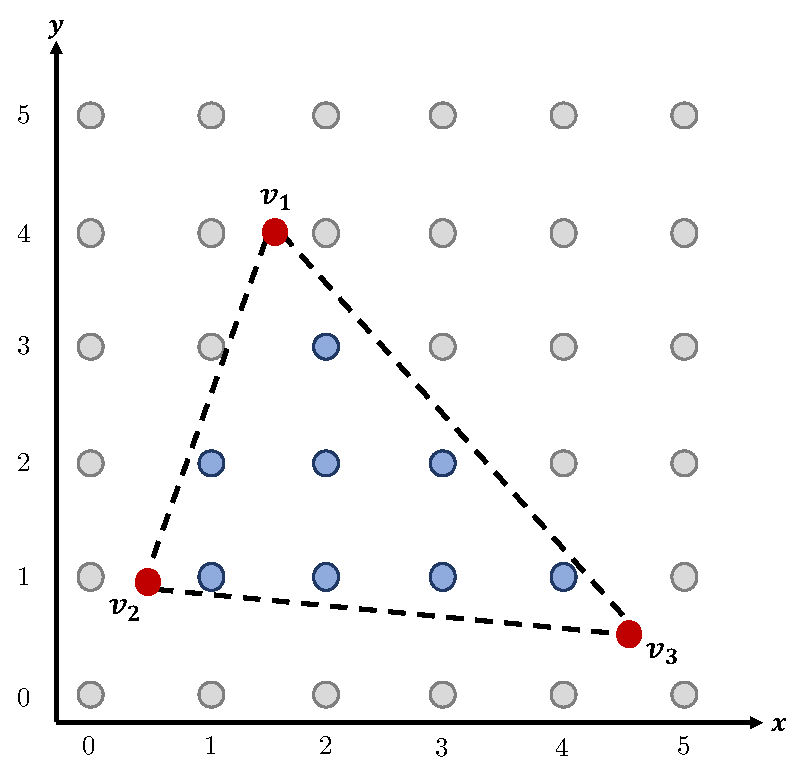
\includegraphics[scale=0.6]{imgs/shader}
\end{figure}

 Given parameters of the three vertices:

\begin{itemize}
\item \textbf{vertex coordinates in window space:} $\vec{v_1}$ = (1.5,\ 4),  $\vec{v_2}$ = (0.5,\ 1), $\vec{v_3}$ = (4.5,\ 0.5)
\item \textbf{depth values in window space with range $[0,\ 1]$:} $z_{1}$ = 0.7, $z_{2}$ = 0.5, $z_{3}$ = 0.3
\item \textbf{normals in view space:} $\vec{n}_1 = (-\frac{2}{3},\ \frac{2}{3},\ \frac{1}{3})^T$, $\vec{n}_2 = (-\frac{2}{3},\ -\frac{2}{3},\ \frac{1}{3})^T$, $\vec{n}_3 = (\frac{2}{3},\ -\frac{2}{3},\ \frac{1}{3})^T$
\end{itemize}


\begin{enumerate}[label=(\roman*)]
\itemsep1em
\item Compute 3D coordinates of all three vertices in view space, given the following parameters: \points{15}
\begin{itemize}
\item \textit{aspect} = $\frac{\text{width}}{\text{height}}$ = 1
\item \textit{fovy} = $90^\circ$
\item \textit{zNear} = 2, \textit{zFar} = 22
\end{itemize}
Note that projection matrix can be constructed as follows.
$$M_{proj} = \begin{pmatrix}
1 & 0 & 0 & 0 \\
0 & 1 & 0 & 0 \\
0 & 0 & -\frac{6}{5} & -\frac{22}{5} \\
0 & 0 & -1 & 0
\end{pmatrix}$$
%
and you may use this matrix in your calculation.

\textbf{Hint:} If you have a vector in normalized device coordinates (NDC), you can transform it into clip space by
multiplying $\vec{v}_{ndc}$ by $w_{clip}$ and plugging in $w_{clip}$ as the fourth element. The problem is that we do not know $w_{clip}$ directly. However, we can compute it from $z_{ndc}$ and certain portions of the projection matrix. Assume that the projection matrix has the following structure
%
$$M_{proj} = \begin{pmatrix}
\star & \star & \star & \star \\
\star & \star & \star & \star \\
0 & 0 & T_1 & T_2 \\
0 & 0 & E_1 & 0
\end{pmatrix},$$
%
where $\star$ denotes elements that are not being used. Since we know
%
$$z_{clip} = T_1\times z_{view} + T_2$$
$$w_{clip} = E_1\times z_{view}$$
$$z_{ndc} = z_{clip} / w_{clip}$$
Then we can find $w_{clip}$ as follows.
$$w_{clip} = \frac{T_2}{z_{ndc} - \frac{T_1}{E_1}}$$
%
The derivation is not covered here, but you are encouraged to derive it by yourself; this will not be graded.

\item Compute the color of each vertex using the Phong lighting model given the following conditions: \points{10}
\begin{itemize}
\item point light source located at $\vec{l}$ = (5,\ 5,\ 5) in view space with RGB color $\vec{I} = (10,\ 10,\ 10)^T$
\item diffuse material properties: $\vec{m_{1}} = (1,\ 0,\ 0)^T$, $\vec{m_{2}} = (0,\ 1,\ 0)^T$, $\vec{m_{3}} = (0,\ 0,\ 1)^T$
\item neglect specular and ambient components of lighting
\item consider square distance falloff ($k_c = k_l = 0,\ k_q = 1$)
\end{itemize}
\textbf{Note: } In the Gouraud shading model (i.e., per-vertex lighting), the lighting calculations are done for each vertex similar to what you just calculated. Afterward, the rasterizer will interpolate the color values of the three vertices over the entire triangle (similar in spirit to what you just did). Remember that the Phong shading model (i.e., per-fragment lighting) uses the rasterizer to interpolate the vertex positions and also the normals over the triangle and then performs the lighting calculations per fragment.

In this particular case, Gouraud shading includes lighting calculations for the three vertices whereas Phong shading would require lighting calculations for all eight fragments that are inside this triangle. This would make per-fragment lighting significantly slower.

\item Oftentimes, per-fragment lighting involves more calculations than per-vertex lighting. Are there cases when this is not true? When specifically would Phong shading (i.e., per-fragment lighting) be faster than Gouraud shading (i.e., per-vertex lighting)? \points{5}

\end{enumerate}

%%%%%%%%%%%%%%%%%%
%   Answer #2 
%%%%%%%%%%%%%%%%%%

\begin{answer}
\rule{\textwidth}{0.4pt}
	\textbf{Answer:}
	\begin{enumerate}[label=(\roman*)]
		\item Write your answer to this question here.
		\item Write your answer to this question here.
		\item Write your answer to this question here.
	\end{enumerate}
\rule{\textwidth}{0.4pt}
\end{answer}

\newpage

\section{Programming Part}

\subsubsubsection*{2.1.1.3 Attenuation Factor Observations} \label{sec:attenuation_factor_comparison}
Does enabling attenuation have a major impact on the appearance of the scene? If so, how so?

\begin{answer}
\rule{\textwidth}{0.4pt}
	
	\textbf{Answer:}
	
	Write your answer to this question here.

\rule{\textwidth}{0.4pt}
\end{answer}

\subsubsubsection* {2.2.2.1 Gouraud vs. Phong Shading Comparison} \label{sec:gouraud_vs_phong_comparison}

Compare Gouraud shading to Phong shading. How are they different? What are the benefits and downsides of each shading method? Specifically, comment on both quality of shading and computational load. You don't need to actually measure any runtimes here, just briefly discuss them theoretically.


\begin{answer}
\rule{\textwidth}{0.4pt}
	
	\textbf{Answer:}
	
	Write your answer to this question here.

\rule{\textwidth}{0.4pt}
\end{answer}


\end{document}
